% BYTE SPIne documentation.
% Source reconstructed on 26 November 2026 from the PDF of 29 October 2026
% (the original .tex was lost). Build: latexmk -pdf BYTE_SPIne_Documentation.tex
\documentclass[11pt,a4paper]{article}
\usepackage[utf8]{inputenc}
\usepackage[T1]{fontenc}
\usepackage{lmodern} % vector fonts for T1; without it MiKTeX falls back to bitmap (Type 3) fonts
\usepackage{amsmath}
\usepackage{amssymb}
\usepackage{graphicx}
\usepackage{geometry}
\usepackage{booktabs}
\usepackage{array}
\usepackage{float}
\usepackage{caption}
\usepackage{xcolor}
\usepackage{enumitem}
\usepackage{pdfpages}
\usepackage{siunitx}
\usepackage{tikz}
\usetikzlibrary{arrows.meta,positioning,calc}
\usepackage[most]{tcolorbox}
\usepackage{xurl}
\usepackage[hidelinks]{hyperref}

\definecolor{customblue}{RGB}{30, 69, 114}
\definecolor{reqred}{RGB}{185, 30, 45}

\hypersetup{
    colorlinks=true,
    linkcolor=customblue,
    citecolor=customblue,
    filecolor=customblue,
    urlcolor=customblue,
}

\geometry{a4paper, margin=1in}
\sisetup{range-phrase = {\text{ to }}, range-units = repeat, list-units = repeat}

% Red box for the mandatory points of use
\newtcolorbox{reqbox}{enhanced, colback=reqred!4, colframe=reqred!80!black,
    boxrule=0.5pt, arc=2pt, left=4pt, right=4pt, top=2pt, bottom=2pt}
\newcommand{\required}[1]{\begin{reqbox}\textbf{\color{reqred}Required:} #1\end{reqbox}}
\newcommand{\reqhead}[1]{\textbf{\color{reqred}#1}}

% Blue box for the validation status of the board
\newtcolorbox{statusbox}{enhanced, colback=customblue!5, colframe=customblue,
    boxrule=0.5pt, arc=2pt, left=4pt, right=4pt, top=2pt, bottom=2pt}

\newcommand{\net}[1]{\texttt{#1}}
\newcommand{\sireport}{\href{run:BYTE_SPIne_SI_Simulation.pdf}{SI report}~\cite{si}}

\begin{document}

\begin{titlepage}
    \centering
    \vspace*{2cm}

    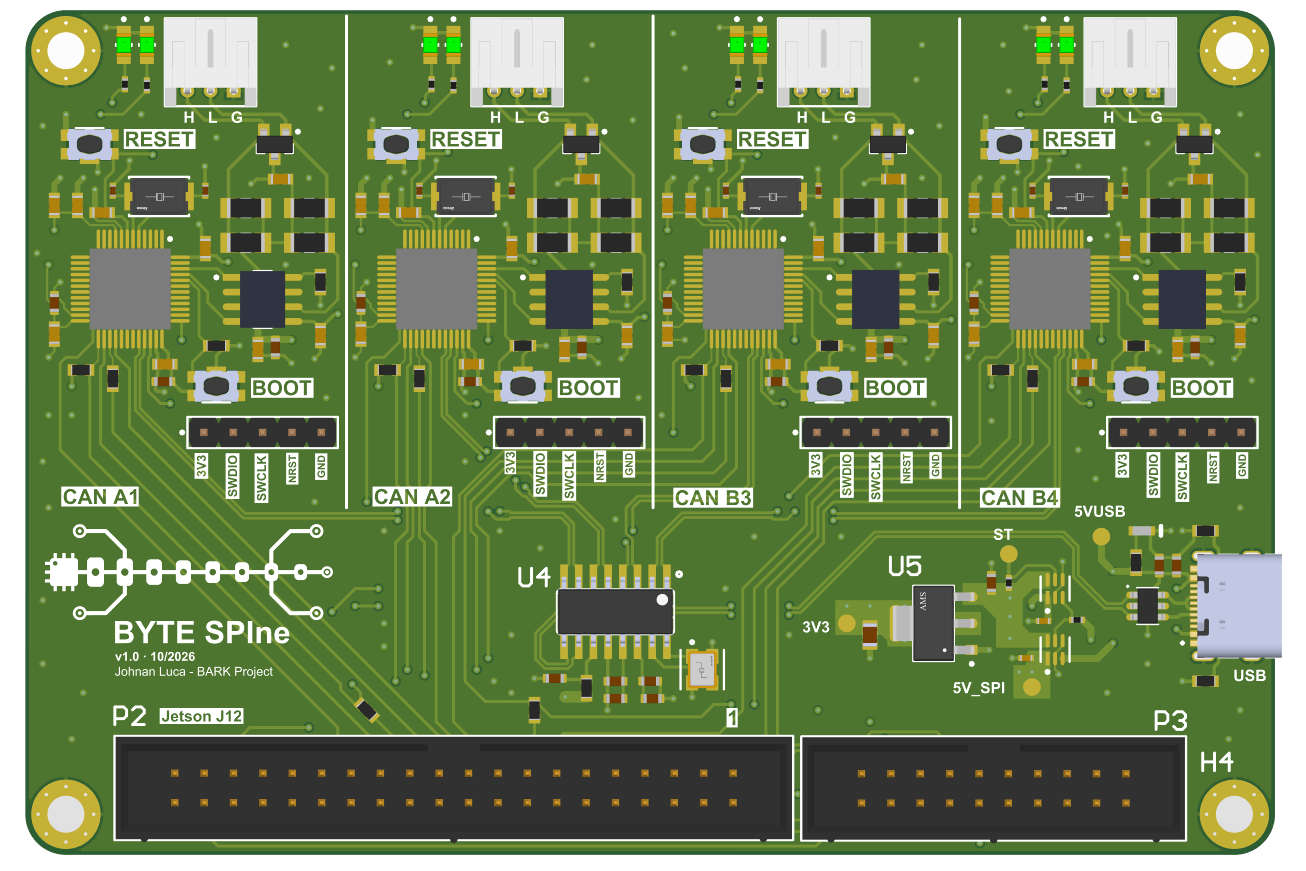
\includegraphics[width=10cm]{BYTE_SPIne_render.png}

    \vspace{2cm}

    {\Huge Architecture Design and Sizing of the\\[4pt] ``BYTE SPIne'' SPI-to-CAN Bridge\par}

    \vspace{1.2cm}

    {\normalsize 29 October 2026 \par}
    {\small Revised 26 November 2026: USB mode validated, SPI mode not yet tested (Section~\ref{sec:next}) \par}

    \vspace{1cm}

    {\large BYTE SPIne version 1.0 \par}

    \vspace{1cm}

    {\normalsize Johnan Luca \par}
    {\normalsize BARK Project - AI Team-Robotics \par}

    \vfill

    {\footnotesize A practical documentation for understanding the BYTE SPIne architecture and the sizing of its
    elements. The impedance and signal integrity simulations are documented in the companion report
    \textit{Impedance and Signal Integrity Simulation of the BYTE SPIne}
    (\href{run:BYTE_SPIne_SI_Simulation.pdf}{\texttt{BYTE\_SPIne\_SI\_Simulation.pdf}}). \par}
\end{titlepage}

\tableofcontents

\vspace{1cm}
\begin{statusbox}
\textbf{\color{customblue}CURRENT STATUS (26 November 2026)}

\smallskip
\begin{itemize}[leftmargin=*, nosep]
    \item \textbf{USB mode (candleLight): tested and validated.} The BYTE SPIne works correctly and
    without errors through the on-board USB hub.
    \item \textbf{SPI mode: not yet tested.} The SPI interface (Section~\ref{sec:miso}--\ref{sec:cubemx}), the SPI
    firmware and the SPI-related bench tests of Section~\ref{sec:next} are still to be verified. The red boxes
    marked \textit{Firmware (SPI mode)} in Section~\ref{sec:req} apply as soon as the SPI mode is used.
\end{itemize}
\end{statusbox}
\newpage

% ---------------------------------------------------------------------------
\section{Abstract and System Overview}

The BYTE SPIne is the communication backbone between the high-level computer of the BARK
quadruped robot, an NVIDIA Jetson Orin Nano, and its twelve joint actuators. Each leg carries
three SteadyWin GIM8108-8 brushless actuators, which are commanded over a classic CAN~2.0
bus (standard 11-bit frames, 8-byte payload, up to \qty{1}{Mbit/s}). The board creates \textbf{four
independent CAN buses}, one per leg, each driven by its own STM32F072C8T6 microcontroller and
TCAN1042HV transceiver.

The board is designed to be operated in two modes on the same hardware:
\begin{itemize}
    \item \textbf{USB mode (development):} the four MCUs are connected to the Jetson through an
    on-board four-port USB hub (SL2.1A). Each MCU runs the open-source \textit{candleLight} firmware
    and appears in Linux as a standard \texttt{gs\_usb} SocketCAN interface (\texttt{can0}--\texttt{can3}). This mode
    allows the robot to be operated immediately, while the SPI firmware is being developed.
    \item \textbf{SPI mode (final):} the four MCUs act as SPI slaves on the two SPI controllers of the
    Jetson 40-pin expansion header. The MCU runs the time-critical CAN loop locally, while
    the Jetson only exchanges setpoints and motor states.
\end{itemize}

\noindent Supporting both modes on one design avoids a second PCB order when moving from USB to
SPI, and makes use of the minimum order quantity of the PCBA service (JLCPCB). All SMD
components are chosen from the JLCPCB assembly catalogue, with priority to \textit{Basic} parts (no
setup fee)~\cite{jlcparts}; this choice drives several sizing decisions in the following sections. The
through-hole connectors are soldered by hand.

The power of the board is drawn from the Jetson itself, either from the USB VBUS or from
the \qty{5}{V} pins of the expansion header, through an ideal-diode OR-ing stage.

\subsection{Requirements for Correct Use}\label{sec:req}

The following points are mandatory to operate the board correctly. They are explained in the
referenced sections and highlighted there in red boxes.

\begin{reqbox}
\reqhead{Wiring and setup}
\begin{enumerate}[leftmargin=*, nosep]
    \item The GND of the SPIne must be common with the ground of the motor power supply
    (Section~\ref{sec:esd}).
    \item On each leg, the CAN termination must be enabled \textbf{only on the last actuator}; all
    actuators must run at \qty{1}{Mbit/s} (Sections~\ref{sec:busload} and~\ref{sec:termination}).
    \item Ribbon cables are connected and disconnected only with the robot switched off
    (Section~\ref{sec:esdjetson}).
    \item At most \qty{0.1}{A} may be drawn from pin~1 of P3, and no further loads may be added to the
    \qty{5}{V} rail (Sections~\ref{sec:p3} and~\ref{sec:budget}).
\end{enumerate}
\reqhead{Jetson}
\begin{enumerate}[leftmargin=*, nosep, resume]
    \item The SPI controllers must be enabled once with \texttt{jetson-io}; SPI clock \qtyrange{1}{4}{MHz},
    ribbon cable shorter than \qtyrange{15}{20}{cm} (Section~\ref{sec:txb}).
\end{enumerate}
\reqhead{Firmware (SPI mode)}
\begin{enumerate}[leftmargin=*, nosep, resume]
    \item Clock from the \qty{8}{MHz} crystal (HSE), Serial Wire debug enabled, SPI and SPI\_INT pins
    at low output speed (Section~\ref{sec:cubemx}).
    \item An MCU whose NSS is high must release MISO (high impedance); to be verified on the
    bench (Section~\ref{sec:miso}).
    \item CRC, sequence counter and communication watchdog must be implemented before the
    robot is operated in SPI mode (Section~\ref{sec:fwarch}).
\end{enumerate}
\end{reqbox}

% ---------------------------------------------------------------------------
\newpage
\section{System Architecture}

\begin{figure}[H]
\centering
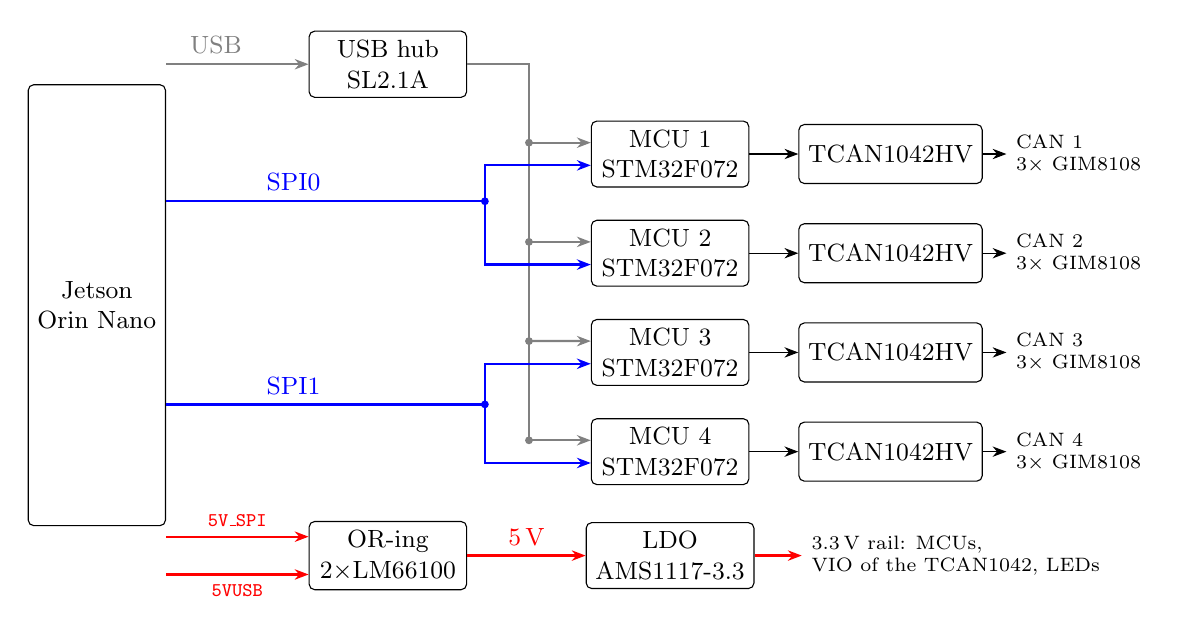
\begin{tikzpicture}[
    font=\small, x=1.12cm, y=1.2cm,
    blk/.style={draw, rounded corners=2pt, align=center, minimum width=2cm, minimum height=0.75cm},
    arr/.style={-{Stealth[length=5pt]}},
    usb/.style={gray, thick},
    spi/.style={blue, thick},
    pwr/.style={red, thick},
    dot/.style={circle, fill, inner sep=1pt}]

    \node[draw, rounded corners=2pt, minimum width=1.6cm, minimum height=5.6cm, align=center]
        (jet) at (0,0.45) {Jetson\\Orin Nano};

    \node[blk] (hub) at (3.3,3.0) {USB hub\\SL2.1A};
    \foreach \i/\y in {1/2.05, 2/1.0, 3/-0.05, 4/-1.1} {
        \node[blk] (mcu\i) at (6.5,\y) {MCU \i\\STM32F072};
        \node[blk] (tc\i) at (9.0,\y) {TCAN1042HV};
        \node[right=0.3cm of tc\i, align=left, font=\scriptsize] (can\i) {CAN \i\\$3\times$ GIM8108};
        \draw[arr] (tc\i) -- (can\i);
        \draw[arr] (mcu\i) -- (tc\i);
        \draw[usb, arr] (4.9,\y+0.12) node[dot, gray] {} -- ($(mcu\i.west)+(0,0.12)$);
    }

    % USB path
    \draw[usb, arr] (jet.east |- hub) -- node[above, pos=0.35] {USB} (hub);
    \draw[usb] (hub.east) -| (4.9,-0.98);

    % SPI buses
    \draw[spi] (jet.east |- 0,1.55) -- node[above, pos=0.4] {SPI0} (4.4,1.55) node[dot] {};
    \draw[spi, arr] (4.4,1.55) |- ($(mcu1.west)+(0,-0.12)$);
    \draw[spi, arr] (4.4,1.55) |- ($(mcu2.west)+(0,-0.12)$);
    \draw[spi] (jet.east |- 0,-0.6) -- node[above, pos=0.4] {SPI1} (4.4,-0.6) node[dot] {};
    \draw[spi, arr] (4.4,-0.6) |- ($(mcu3.west)+(0,-0.12)$);
    \draw[spi, arr] (4.4,-0.6) |- ($(mcu4.west)+(0,-0.12)$);

    % Power
    \node[blk] (or) at (3.3,-2.2) {OR-ing\\$2\times$LM66100};
    \node[blk] (ldo) at (6.5,-2.2) {LDO\\AMS1117-3.3};
    \draw[pwr, arr] (jet.east |- 0,-2.0) -- node[above, font=\scriptsize\ttfamily] {5V\_SPI} (or.west |- 0,-2.0);
    \draw[pwr, arr] (jet.east |- 0,-2.4) -- node[below, font=\scriptsize\ttfamily] {5VUSB} (or.west |- 0,-2.4);
    \draw[pwr, arr] (or) -- node[above] {5\,V} (ldo);
    \node[right=0.6cm of ldo, align=left, font=\scriptsize] (rail) {3.3\,V rail: MCUs,\\VIO of the TCAN1042, LEDs};
    \draw[pwr, arr] (ldo) -- (rail);
\end{tikzpicture}
\caption{Block diagram of the BYTE SPIne. SPI0 serves MCU 1--2, SPI1 serves MCU 3--4; the
USB hub provides the development path (candleLight), with one downstream port per MCU.
The board is supplied by the two \qty{5}{V} sources of the Jetson (\net{5V\_SPI} from the 40-pin header,
\net{5VUSB} from the USB VBUS), combined by the ideal-diode OR-ing into the \qty{5}{V} rail (transceivers,
USB hub, LDO). The LDO generates the \qty{3.3}{V} rail.}
\label{fig:block}
\end{figure}

The schematic is hierarchical. The sheet \texttt{CAN\_channel.SchDoc} describes one complete channel
(MCU, clock, debug, transceiver, termination and protection) and is instantiated four times
through two multi-channel sheet symbols, \texttt{Repeat(CAN\_A,1,2)} and \texttt{Repeat(CAN\_B,3,4)}. Grouping
the channels in pairs mirrors the two SPI buses of the Jetson and keeps the net names unique
(\texttt{SPI0\_*} and \texttt{SPI1\_*}). Component designators therefore carry a channel suffix, e.g.\ \texttt{U1\_CAN\_A1}
or \texttt{C3\_CAN\_B4}.

\subsection{MCU Pin Assignment}

\begin{table}[H]
\centering
\begin{tabular}{lll}
\toprule
STM32F072 pin & Function & Notes \\
\midrule
PA0, PA1   & Status LEDs (green, yellow)  & driven through R1, R2 \\
PA11, PA12 & USB DM, DP                   & to the hub downstream port \\
PA13, PA14 & SWDIO, SWCLK                 & debug header P1 \\
PB8, PB9   & CAN\_RX, CAN\_TX             & AF4, bxCAN \\
PB11       & SPI\_INT (GPIO output)       & data-ready line to the Jetson \\
PB12--PB15 & SPI2 NSS, SCK, MISO, MOSI    & SPI slave \\
PF0, PF1   & OSC\_IN, OSC\_OUT            & \qty{8}{MHz} crystal \\
BOOT0      & Boot selection               & button S1, pull-down R10 \\
NRST       & Reset                        & button S2, C4 \\
\bottomrule
\end{tabular}
\caption{Pin assignment of each MCU channel.}
\label{tab:pins}
\end{table}

% ---------------------------------------------------------------------------
\newpage
\section{Microcontroller Subsystem (STM32F072C8T6)}

\subsection{Clock Source: Why an External Crystal}\label{sec:clock}

The STM32F072 is a crystal-less USB device: in USB mode its internal \qty{48}{MHz} oscillator (HSI48)
is trimmed continuously by the Clock Recovery System using the USB start-of-frame packets.
This is not sufficient for CAN. When the board runs in SPI mode, no USB host is present and
the internal oscillators are untrimmed. The datasheet~\cite{stm32} specifies:
\begin{itemize}
    \item HSI (\qty{8}{MHz}): $\pm\qty{1}{\percent}$ at \qty{25}{\degreeCelsius}, $-2.8/+\qty{3.8}{\percent}$ over \qty{-40}{\degreeCelsius} to \qty{105}{\degreeCelsius};
    \item HSI48 (factory calibrated): $-2.8/+\qty{2.9}{\percent}$ at \qty{25}{\degreeCelsius}, $-4.9/+\qty{4.7}{\percent}$ over the full range.
\end{itemize}
A CAN network at \qty{1}{Mbit/s} typically tolerates an oscillator error well below \qty{1}{\percent}. An \qty{8}{MHz}
crystal (YXC X50328MSB2GI, $\pm\qty{10}{ppm}$, $C_L = \qty{20}{pF}$) is therefore mounted on PF0/PF1. The
crystal also feeds the PLL for USB, so both modes work from the same clock tree.

\subsection{Crystal Load Capacitors}

Following AN2867~\cite{an2867}, the two load capacitors appear in series as seen by the crystal, in parallel
with the stray capacitance of pins and traces ($C_{stray} \approx \qtyrange{3}{5}{pF}$):
\begin{equation}
C_L = \frac{C_7\,C_8}{C_7 + C_8} + C_{stray} \quad\Rightarrow\quad
C_7 = C_8 = 2\,(C_L - C_{stray}) = 2\,(20 - 3.5)\,\unit{pF} \approx \qty{33}{pF}
\end{equation}
With the selected \qty{33}{pF} C0G capacitors the effective load is $16.5 + (3\dots5) = \qtyrange{19.5}{21.5}{pF}$,
centred on the \qty{20}{pF} specification of the crystal.

\subsection{Power Supply Decoupling}

The decoupling follows the power supply scheme of the datasheet~\cite{stm32} (figure 13) and of
AN4080~\cite{an4080}: one \qty{100}{nF} capacitor per VDD pin plus one common \qty{4.7}{\micro F}, a dedicated \qty{100}{nF}
+ \qty{4.7}{\micro F} pair on VDDIO2, and \qty{10}{nF} + \qty{1}{\micro F} on VDDA. All capacitors are on the \qty{3.3}{V} net, so
their assignment to a pin is defined by the placement:
\begin{itemize}
    \item VDD pin 24: C14 (\qty{100}{nF}) and C13 (\qty{4.7}{\micro F}, common VDD bulk);
    \item VDD pin 48 (and VBAT, pin 1, at the same corner): C10 (\qty{100}{nF});
    \item VDDIO2 pin 36: C15 (\qty{100}{nF}) and C5 (\qty{4.7}{\micro F});
    \item VDDA pin 9: C11 (\qty{10}{nF}, closest to the pin) and C12 (\qty{1}{\micro F}).
\end{itemize}
The \qty{100}{nF} capacitors must sit directly at their pins, because they supply the fast current edges.
The \qty{4.7}{\micro F} bulk capacitors cover slow load changes and are much less sensitive to their position:
they reach the other pins through the \qty{3.3}{V} and GND planes, whose inductance is about \qty{1}{nH}
(\qty{6}{m\ohm} at \qty{1}{MHz}).

\subsection{Boot, Reset and Debug}

BOOT0 is held low by R10 (\qty{10}{k\ohm}); pressing S1 at reset pulls it to \qty{3.3}{V} and starts the ST system
bootloader (USB DFU), which is the standard way to flash candleLight. NRST is filtered by
C4 (\qty{100}{nF}) against the internal pull-up of about \qty{40}{k\ohm}; S2 provides a manual reset. The frame
terminal (pin 5) of both KMR221G buttons is tied to GND for ESD.

Each channel exposes a 5-pin SWD header P1 (3V3, SWDIO, SWCLK, NRST, GND) for
programming and debugging with an ST-Link, independently of USB. The open-drain reset
output of the probe is compatible with C4.

% ---------------------------------------------------------------------------
\newpage
\section{CAN Physical Layer}

\subsection{Transceiver: TCAN1042HV}

The TCAN1042HVDR is supplied with $V_{CC} = \qty{5}{V}$ (recommended range \qtyrange{4.5}{5.5}{V}) and
uses the VIO pin at \qty{3.3}{V} (range \qtyrange{3.0}{5.5}{V}) to match the logic levels of the STM32 without
external level shifters. Its bus pins withstand faults up to $\pm\qty{58}{V}$, which is relevant in a robot
where motor supply lines run next to the CAN wiring. The STB pin is tied to GND through
R5 (\qty{10}{k\ohm}) so the device is always in normal mode; the internal pull-up of STB draws at most
\qty{20}{\micro A}, giving less than \qty{0.2}{V} on the pin.

Decoupling: \qty{4.7}{\micro F} + \qty{100}{nF} on VCC (C1, C2), \qty{100}{nF} on VIO (C6).

\subsection{Bus Topology and Bus Load}\label{sec:busload}

Each bus connects the SPIne (first node) to the three actuators of one leg. The GIM8108-8
drivers~\cite{steadywin} use standard 11-bit frames with an 8-byte payload in a request/response scheme, i.e.
two frames per motor per control cycle. A standard frame with 8 data bytes is 111 bits long
without bit stuffing and up to about 135 bits in the worst case:
\begin{equation}
t_{frame} = \frac{111\dots135\ \text{bit}}{\qty{1}{Mbit/s}} = \qtyrange{111}{135}{\micro s}
\end{equation}
\begin{equation}
t_{cycle} = 3\ \text{motors} \times 2\ \text{frames} \times t_{frame} = \qtyrange{0.67}{0.81}{ms}
\end{equation}
At a \qty{1}{kHz} control rate the bus load is therefore \qtyrange{67}{81}{\percent}, at \qty{500}{Hz} it is \qtyrange{33}{41}{\percent}. A
\qty{1}{kHz} loop is feasible only because each leg has its own bus, and requires all actuators to be
configured at \qty{1}{Mbit/s}.

\required{configure \textbf{all actuators of the bus at} \qty{1}{Mbit/s}.}

\subsection{Split Termination Sizing}\label{sec:termination}

A CAN bus must be terminated with \qty{120}{\ohm} at both physical ends. Since the SPIne is always the
first node of each bus, the termination is placed on the board; the last actuator of each leg must
provide the other one, and the intermediate actuators must have their termination disabled.

\required{on each leg, enable the CAN termination \textbf{only on the last actuator} of the bus
and disable it on the intermediate ones.}

The termination is split in two halves of \qty{60}{\ohm} with the centre tap connected to GND through
$C_{split} = \qty{4.7}{nF}$ (C3). This stabilises the common-mode voltage and reduces emissions. Each half
is built from \textbf{two \qty{120}{\ohm} 1206 resistors in parallel} (R6/R15 and R7/R16):
\begin{equation}
R_{half} = \frac{\qty{120}{\ohm}}{2} = \qty{60}{\ohm}, \qquad R_{term} = 2\,R_{half} = \qty{120}{\ohm}
\end{equation}

\paragraph{Why four identical resistors.} At first sight four resistors, two in parallel and the two pairs
in series, look unnecessary: one \qty{60}{\ohm} resistor per half would give the same \qty{120}{\ohm}. The reason is
cost. Each half must withstand the fault power computed below (\qty{0.6}{W} peak), which requires a
large package (2010 or 2512) for a single resistor. In the JLCPCB assembly catalogue~\cite{jlcparts} such
resistors are only available as \textit{Extended} parts, which add a setup fee per part type and a higher
unit price. A \qty{120}{\ohm} 1206 resistor (\qty{0.25}{W}) is instead a \textit{Basic} part, without setup fee. Two of
them in parallel give exactly \qty{60}{\ohm} and double the power rating to \qty{0.5}{W} per half. The price is
one extra small resistor per half, which costs much less than an Extended part.

\paragraph{Normal operation.} The dominant differential voltage is at most $V_{OD(DOM)} = \qty{3}{V}$
(TCAN1042 datasheet~\cite{tcan}, $R_L = \qtyrange{50}{65}{\ohm}$), i.e.\ \qty{1.5}{V} on each half:
\begin{equation}
P_{half} = \frac{(\qty{1.5}{V})^2}{\qty{60}{\ohm}} = \qty{37.5}{mW}, \qquad
P_{resistor} = \frac{P_{half}}{2} \approx \qty{19}{mW}
\end{equation}
This is a peak value during dominant bits; the average is lower.

\paragraph{Fault condition.} The datasheet~\cite{tcan} (section 9.3.6) requires the termination to be sized for bus
fault cases. If a bus line is shorted to a supply rail while the node transmits a dominant bit, the
current is limited by the driver to $I_{OS(SS\_DOM)} \leq \qty{100}{mA}$:
\begin{equation}
P_{half,fault} = I_{OS}^2 \times R_{half} = (\qty{0.1}{A})^2 \times \qty{60}{\ohm} = \qty{0.6}{W}, \qquad
P_{resistor,fault} = \qty{0.3}{W}
\end{equation}
This is a peak value: the average is reduced by the ratio of recessive bits and by the TXD
dominant time-out of the transceiver. A single \qty{60.4}{\ohm} 0603 resistor (\qty{100}{mW}) would not survive
this case; the chosen arrangement provides \qty{0.5}{W} per half using only JLCPCB Basic parts
(\texttt{C17909}).

\subsection{ESD Protection}\label{sec:esd}

A Nexperia PESD1CAN (D1)~\cite{pesd} protects both lines: pins 1 and 2 (cathodes) are connected to
CANH and CANL, pin 3 (common) to GND. The connector J1 is a JST PH 3-pin (S3B-PH-K-S)
with the pinout 1 = GND, 2 = CANL, 3 = CANH.

\required{the GND of the SPIne must be \textbf{common with the ground of the motor
power supply}; without a common reference the CAN common-mode range can be exceeded.}

% ---------------------------------------------------------------------------
\section{SPI Interface to the Jetson Orin Nano}

\subsection{Bus Mapping}

The Jetson Orin Nano developer kit exposes two SPI controllers on the 40-pin header J12~\cite{jetson, jetsonhacks},
each with two hardware chip selects. The four MCUs are therefore split in two pairs, so that
each MCU has a dedicated hardware chip select and each MISO line is shared by only two slaves.

\begin{table}[H]
\centering
\begin{tabular}{llccc}
\toprule
Channel & Jetson bus & SCK / MOSI / MISO (pin) & NSS (pin) & INT (pin) \\
\midrule
CAN\_A1 & SPI0 & 23 / 19 / 21 & 24 (CS0) & 29 \\
CAN\_A2 & SPI0 & 23 / 19 / 21 & 26 (CS1) & 31 \\
CAN\_B3 & SPI1 & 13 / 37 / 22 & 18 (CS0) & 32 \\
CAN\_B4 & SPI1 & 13 / 37 / 22 & 16 (CS1) & 33 \\
\bottomrule
\end{tabular}
\caption{Mapping between the MCU channels and the Jetson 40-pin header (P2). \qty{5}{V} on pins 2
and 4; GND on pins 6, 9, 14, 20, 25, 30, 34, 39. The \qty{3.3}{V} pins 1 and 17 (\net{3V3\_Jetson}) are not
connected to the \qty{3.3}{V} rail of the board: they are only routed to the breakout header P3.}
\label{tab:spimap}
\end{table}

The connection uses a shrouded $2{\times}20$ box header (P2) and a 40-way IDC ribbon cable, so
that the cable cannot be inserted reversed.

\subsection{Breakout Header P3}\label{sec:p3}

The SPIne occupies most of the Jetson header. To keep the remaining Jetson signals usable
(sensors, debug UART, I2S), they are routed one-to-one to a $2{\times}10$ shrouded header P3 (Würth
61202021621):

\begin{table}[H]
\centering
\begin{tabular}{rl|rl}
\toprule
Pin & Signal (J12 pin) & Pin & Signal (J12 pin) \\
\midrule
1  & 3V3\_Jetson (1, 17) & 2  & GND \\
3  & I2C1\_SDA (3)       & 4  & I2C1\_SCL (5) \\
5  & I2C0\_SDA (27)      & 6  & I2C0\_SCL (28) \\
7  & GND                 & 8  & GND \\
9  & UART1\_TXD (8)      & 10 & UART1\_RXD (10) \\
11 & UART1\_RTS (11)     & 12 & UART1\_CTS (36) \\
13 & GND                 & 14 & GPIO09 (7) \\
15 & GPIO12 / PWM (15)   & 16 & I2S0\_SCLK (12) \\
17 & I2S0\_FS (35)       & 18 & I2S0\_DIN (38) \\
19 & I2S0\_DOUT (40)     & 20 & GND \\
\bottomrule
\end{tabular}
\caption{Pinout of the breakout header P3. The \qty{5}{V} rail is not exported on P3: the \qty{0.5}{A} budget
of the Jetson header is reserved for the SPIne.}
\label{tab:p3}
\end{table}

\required{P3 pin 1 (\net{3V3\_Jetson}) is limited to \qty{0.1}{A} by the Jetson; sensors connected to
P3 must stay within this budget or be supplied separately.}

\subsection{ESD Protection of the Jetson Connectors}\label{sec:esdjetson}

ESD protection is placed only on the connectors exposed to handling or to external cables: the
USB-C port (USBLC6-2SC6) and the four CAN connectors (PESD1CAN). P2 and P3 are not
protected on purpose:
\begin{itemize}
    \item P2 is an internal board-to-board connection to the Jetson through a short ribbon cable
    inside the robot, connected only during assembly; the header signals already pass through
    the TXB0108 translators of the carrier board;
    \item a TVS array on the SPI lines would add capacitance to signals that are already at about
    \qty{40}{pF}, while the TXB0108 is sensitive to capacitive loads;
    \item P3 is intended for sensors inside the robot with short cables. If it is ever used with long
    or external cables, the protection should be placed on the sensor side or on an adapter, or
    added in a later revision.
\end{itemize}

\required{connect and disconnect the ribbon cables \textbf{only with the robot switched off},
and handle the boards with ESD precautions.}

\subsection{Level Translators on the Jetson Side}\label{sec:txb}

According to the carrier board specification (SP-11324-001)~\cite{jetson}, all header signals are \qty{3.3}{V} and
pass through TI TXB0108 auto-direction translators~\cite{txb}, whose output drivers are very weak.
NVIDIA requires any pull-up or pull-down on these signals to be weaker than \qty{50}{k\ohm}. For this
reason:
\begin{itemize}
    \item the NSS pull-up R3 is \qty{100}{k\ohm} (not the usual \qty{10}{k\ohm}). It keeps each slave deselected when
    the cable is unplugged (USB mode) or while the Jetson boots;
    \item the internal pull-up of the STM32 (\qtyrange{25}{55}{k\ohm}) is not used for NSS, as it could fall
    below the limit;
    \item the SPI clock should be kept in the range \qtyrange{1}{4}{MHz} and the ribbon cable short
    (below \qtyrange{15}{20}{cm}).
\end{itemize}

\required{the SPI pins of the Jetson are configured as GPIO by default: \textbf{enable the two
SPI controllers once with \texttt{jetson-io}} (\texttt{sudo /opt/nvidia/jetson-io/jetson-io.py},
then reboot). Keep the SPI clock in the range \qtyrange{1}{4}{MHz} and the ribbon cable shorter
than \qtyrange{15}{20}{cm}.}

\subsection{Data Rate and Shared MISO}\label{sec:miso}

Each MCU exchanges roughly 100 bytes per millisecond (three motors, command and state), i.e.
below \qty{1}{Mbit/s}; a \qtyrange[range-phrase=--, range-units=single]{2}{4}{MHz} SPI clock leaves a wide margin. A series resistor R4 (\qty{33}{\ohm}) on MISO
limits the current in case two slaves drive the line at the same time; placed at the MCU pin, it
also works as a source termination of the line (Section~\ref{sec:si}).

\paragraph{Series resistors on SCK.} The two SCK lines also have a \qty{33}{\ohm} series resistor, R17 (SPI1\_SCK)
and R18 (SPI0\_SCK), placed at the Jetson side of the line, next to P2. The TXB0108 translators
of the Jetson drive very fast edges (\qtyrange{0.6}{2.5}{ns}), so the clock line of each bus, which branches
to two MCUs, behaves as a transmission line: every edge is reflected at the ends of the branches
and returns as ringing. Without the resistor, the first ring after the rising edge falls below the
guaranteed $V_{IH}$ of the STM32, so the clock level is no longer guaranteed to be read correctly
during the ring. The series resistor, together with the low output impedance of the driver,
matches the line at the source and damps these reflections. This was found with the signal
integrity simulation of the routed board, which also gives the value of the resistor (\sireport,
Section 3.8); the results are summarised in Section~\ref{sec:si}.

\required{the SPI firmware must guarantee that an MCU whose NSS is high \textbf{releases
MISO} (high impedance). This must be verified on the bench with two MCUs on the same
bus before the full system test.}

\subsection{Recommended Firmware Architecture}\label{sec:fwarch}

The Jetson runs a standard (non real-time) Linux kernel, so SPI transfers can occasionally be
delayed by milliseconds. The design assumes that:
\begin{itemize}
    \item the MCU owns the fast CAN loop, timed by its own timer, and keeps using the last valid
    setpoint if a packet is late;
    \item SPI packets have a fixed length, a hardware CRC and a sequence counter, and are handled
    with circular DMA;
    \item a communication watchdog puts the motors in a safe state (zero torque or damping) if no
    valid packet arrives within a few milliseconds;
    \item the PREEMPT\_RT kernel available for JetPack is used on the Jetson for the final system.
\end{itemize}

\subsection{MCU Peripheral Configuration (STM32CubeMX)}\label{sec:cubemx}

The SPI-mode firmware must configure the peripherals explicitly; the pins of the SPI2 controller
are plain GPIOs after reset. This configuration is not needed in USB mode, where candleLight
provides its own board configuration.

\begin{table}[H]
\centering
\begin{tabular}{l>{\raggedright\arraybackslash}p{0.74\textwidth}}
\toprule
Peripheral & Configuration \\
\midrule
RCC (clock) & HSE \qty{8}{MHz} crystal (PF0 = OSC\_IN, PF1 = OSC\_OUT) $\to$ PLL $\times 6$ $\to$
SYSCLK = HCLK = PCLK = \qty{48}{MHz}. The HSE is mandatory for an
accurate CAN bit rate (Section~\ref{sec:clock}). \\
SPI2 & Mode \textit{Full-Duplex Slave}, \textit{Hardware NSS Input Signal} (on PB12); 8-bit data,
MSB first; CPOL/CPHA identical to the Jetson (spidev default: mode 0,
CPOL = 0, CPHA = 0); RX and TX on DMA in circular mode (CubeMX
assigns SPI2\_RX/TX to DMA1 channels 4/5). \\
SPI2 pins & PB12 = NSS, PB13 = SCK, PB14 = MISO, PB15 = MOSI; alternate
function AF0, no internal pull (R3 provides the external \qty{100}{k\ohm} pull-up on
NSS), \textbf{low output speed}. \\
Packet integrity & CRC computed on each packet with the CRC peripheral of the STM32F072
(programmable polynomial), so that the Jetson can compute the same value
in software. The built-in SPI CRC is an alternative, but with circular DMA
it requires the Jetson to append a matching CRC at the end of every frame. \\
bxCAN & PB8 = CAN\_RX, PB9 = CAN\_TX; alternate function AF4. \qty{1}{Mbit/s}
from PCLK = \qty{48}{MHz}: prescaler 3 ($t_q = \qty{62.5}{ns}$), SJW = 1, BS1 = 13\,$t_q$,
BS2 = 2\,$t_q$, i.e.\ 16\,$t_q$ per bit and a sample point of \qty{87.5}{\percent}. \\
GPIO & PB11 = SPI\_INT: push-pull output, low speed, initialised to the inactive
level. PA0 = green LED, PA1 = yellow LED: push-pull outputs. \\
SYS & Debug \textit{Serial Wire} enabled (PA13 = SWDIO, PA14 = SWCLK), otherwise
CubeMX may release the pins and the SWD probe loses access. \\
IWDG & Independent watchdog (LSI) for MCU lock-ups, in addition to the communication
watchdog implemented in software. \\
\bottomrule
\end{tabular}
\caption{STM32CubeMX configuration of each MCU for the SPI-mode firmware.}
\label{tab:cubemx}
\end{table}

\required{in the SPI firmware, the clock must come from the \textbf{HSE crystal}, the debug
interface must stay enabled (\textbf{Serial Wire}) and the SPI and SPI\_INT pins must be at \textbf{low
output speed}.}

\textbf{Hardware note:} in slave mode the MISO output must be in high impedance while NSS is
high, otherwise the two MCUs of a bus drive MISO at the same time. This is the bench test
listed in the next steps (Section~\ref{sec:next}); if the peripheral does not release the pin, the firmware must
switch PB14 between alternate function and input on the NSS edges (EXTI on PB12).

% ---------------------------------------------------------------------------
\section{USB Subsystem}

\subsection{USB Type-C Upstream Port}

J2 (TYPE-C-31-M-12) is configured as a USB 2.0 device (UFP): CC1 and CC2 are pulled down
with \qty{5.1}{k\ohm} (R11, R12) so that the host enables VBUS. D+ and D$-$ are protected by a USBLC6-2SC6
(U3) placed close to the connector. VBUS is decoupled with \qty{10}{\micro F} + \qty{100}{nF}, keeping the
total bulk capacitance at the \qty{10}{\micro F} limit for a USB device. A red LED (DS1, R13 = \qty{1}{k\ohm})
indicates the presence of VBUS.

\subsection{USB Hub: SL2.1A}

The SL2.1A is a single-supply USB 2.0 four-port hub with internal \qty{3.3}{V} and \qty{1.8}{V} regulators.
Following the reference circuit of its datasheet~\cite{sl21a}:
\begin{itemize}
    \item VDD33 (pin 13) and VDD18 (pin 14): \qty{4.7}{\micro F} + \qty{100}{nF} each (C9/C16, C17/C18), placed
    as close as possible to the pins;
    \item VCC5V (pin 11): RC filter made of R8 = \qty{4.7}{\ohm} and C19 = \qty{4.7}{\micro F};
    \item crystal Y2: \qty{12}{MHz}, $C_L = \qty{20}{pF}$, $\leq\qty{20}{ppm}$ (YXC X322512MSB4SI, $\pm\qty{10}{ppm}$). No load
    capacitors are required by the SL2.1A.
\end{itemize}
The four downstream ports are routed directly to the USB pins of the four MCUs.

\subsection{candleLight Firmware}

In USB mode each STM32F072 runs candleLight (\texttt{candle-usb/candleLight\_fw})~\cite{candlelight}, whose
reference hardware uses the same MCU with CAN on PB8/PB9. The Linux \texttt{gs\_usb} driver
exposes each channel as a SocketCAN interface, so no driver needs to be written on the Jetson
side.

% ---------------------------------------------------------------------------
\section{Power Architecture}

\subsection{Ideal-Diode OR-ing (LM66100)}

The board can be powered from two \qty{5}{V} sources of the Jetson: \net{5V\_SPI} (header pins 2 and 4)
and \net{5VUSB} (USB VBUS). A Schottky OR-ing would drop \qtyrange{0.4}{0.5}{V} at the board current;
starting from a USB VBUS of \qty{4.75}{V}, this would leave about \qty{4.3}{V}, below the \qty{4.5}{V} minimum of
the TCAN1042 (whose VCC undervoltage protection rises at \qtyrange{4.2}{4.4}{V}). Two TI LM66100
ideal diodes are used instead:
\begin{equation}
V_{drop} = I \times R_{ON} = \qty{0.43}{A} \times \qty{79}{m\ohm} \approx \qty{34}{mV}, \qquad
P = I^2 R_{ON} \approx \qty{15}{mW}
\end{equation}

Since both sources come from the same internal rail of the Jetson (VDD\_5V\_SYS), their
voltages are almost identical. The simple cross-coupled OR-ing (LM66100 datasheet~\cite{lm66100}, figure
15) can switch both devices off in this condition. The circuit therefore implements figure 17,
`Dual Ideal Diode ORing for Continuous Output Power':
\begin{itemize}
    \item U6 (priority, \net{5V\_SPI}): CE connected to \net{5VUSB}; ST pulled up to \net{5V\_SPI} by R9 (\qty{100}{k\ohm}) and
    connected to the CE of U7;
    \item U7 (secondary, \net{5VUSB}): CE driven by the ST of U6; ST pulled up to \qty{5}{V} by R14 and
    brought to test point TP2.
\end{itemize}

\begin{table}[H]
\centering
\begin{tabular}{l>{\raggedright\arraybackslash}p{0.72\textwidth}}
\toprule
Scenario & Behaviour \\
\midrule
Only \net{5V\_SPI} & U6 on (its CE sees \qty{0}{V}), ST of U6 high-Z, R9 pulls CE of U7 high: U7 off. \\
Only \net{5VUSB} & U6 unpowered, pull-up R9 at \qty{0}{V}: CE of U7 low, U7 on. \\
Both present & U6 has priority; if U6 switches off because the inputs are equal, its ST goes
low and enables U7 immediately, so the output is never left unpowered. \\
\bottomrule
\end{tabular}
\caption{Operating scenarios of the OR-ing stage. TP2 (ST of U7) reads high when U7 is
conducting.}
\label{tab:oring}
\end{table}

Each LM66100 has a \qty{1}{\micro F} input capacitor (C24, C25).

\subsection{\texorpdfstring{\qty{3.3}{V}}{3.3 V} Regulator (AMS1117-3.3)}

The \qty{3.3}{V} rail supplies the four MCUs, the VIO pins of the transceivers and the LEDs. With
a typical MCU current of \qty{24}{mA} at \qty{48}{MHz} (datasheet~\cite{stm32}, all peripherals enabled) the load is
about \qty{150}{mA}:
\begin{equation}
P_{LDO} = (V_{IN} - V_{OUT}) \times I = (4.95 - 3.3)\,\unit{V} \times \qty{0.15}{A} \approx \qty{0.25}{W}
\end{equation}
which is easily handled by the SOT-223 package. The dropout (\qty{1.1}{V} at \qty{0.8}{A}, lower at this
current) requires $V_{IN} \gtrsim \qty{4.4}{V}$, which the ideal-diode OR-ing preserves.

\textbf{Hardware note:} the AMS1117 datasheet~\cite{ams1117} guarantees stability for all conditions with a
\qty{22}{\micro F} solid tantalum output capacitor. The design uses a \qty{22}{\micro F} 0805 \qty{25}{V} X5R ceramic capacitor
(C21), a common and generally stable choice. The \qty{3.3}{V} rail must be checked for oscillation with
an oscilloscope on the prototype; if needed, C21 can be replaced by a tantalum capacitor.

\subsection{Current Budget}\label{sec:budget}

\begin{table}[H]
\centering
\begin{tabular}{lr}
\toprule
Load & Current (worst case) \\
\midrule
$4\times$ TCAN1042 (dominant, $R_L = \qty{60}{\ohm}$, max) & \qty{280}{mA} \\
\qty{3.3}{V} rail through the LDO (4 MCUs, LEDs, VIO) & \qty{150}{mA} \\
USB hub and VBUS LED (estimate) & \qty{30}{mA} \\
\midrule
Total on the \qty{5}{V} rail & $\approx\qty{0.46}{A}$ \\
\bottomrule
\end{tabular}
\caption{Worst-case current budget. In normal operation the transceivers draw \qty{2.5}{mA} in the
recessive state, so the typical current is significantly lower.}
\label{tab:budget}
\end{table}

\required{the Jetson carrier board specification limits the \qty{5}{V} current to \qty{0.5}{A} for the 40-pin
header and \qty{0.5}{A} per USB port. The worst case is within this limit with little margin:
\textbf{no further loads may be added to the \qty{5}{V} rail}.}

% ---------------------------------------------------------------------------
\section{LEDs}

\subsection{LED Resistor Sizing}

The series resistor of each LED is sized with Ohm's law:
\begin{equation}
R = \frac{V_{rail} - V_f}{I_f} \quad\iff\quad I_f = \frac{V_{rail} - V_f}{R}
\end{equation}

\begin{table}[H]
\centering
\begin{tabular}{llllll}
\toprule
LED & Part & Rail & $V_f$ & $R$ & $I_f$ \\
\midrule
D2 green  & KT-0805G & \qty{3.3}{V} (PA0) & \qtyrange{2.6}{3.1}{V} & \qty{100}{\ohm} & \qtyrange{2}{7}{mA} \\
D3 yellow & KT-0805Y & \qty{3.3}{V} (PA1) & \qtyrange{1.8}{2.4}{V} & \qty{1}{k\ohm} & \qtyrange{0.9}{1.5}{mA} \\
DS1 red   & KT-0603R & \qty{5}{V} (VBUS)  & \qtyrange{1.8}{2.4}{V} & \qty{1}{k\ohm} & \qtyrange{2.6}{3.2}{mA} \\
\bottomrule
\end{tabular}
\caption{LED operating points. The green LED has a high forward voltage: with \qty{1}{k\ohm} it would
be almost off at \qty{3.3}{V}, hence the \qty{100}{\ohm} resistor.}
\label{tab:leds}
\end{table}

\subsection{BYTE SPIne LEDs Color Code}
\begin{itemize}[nosep]
    \item \textbf{RED (DS1):} USB VBUS present.
    \item \textbf{GREEN (D2, per channel):} MCU status / CAN activity (defined by the firmware).
    \item \textbf{YELLOW (D3, per channel):} MCU status / CAN activity (defined by the firmware).
\end{itemize}

% ---------------------------------------------------------------------------
\newpage
\section{PCB Layout}

\subsection{Stack-up}

The board uses the standard JLCPCB 4-layer stack-up JLC04161H-7628 (\qty{1.6}{mm})~\cite{jlcstack}. Signals
are routed on the outer layers; the two inner layers are reference and distribution planes.

\begin{table}[H]
\centering
\begin{tabular}{llll}
\toprule
Layer & Function & Copper & Dielectric to next layer \\
\midrule
L1 Top    & signals, components         & \qty{35}{\micro m} (1\,oz)    & prepreg \qty{0.2104}{mm}, $\varepsilon_r = 4.4$ \\
L2 GND    & solid GND plane             & \qty{15.2}{\micro m} (0.5\,oz) & core \qty{1.065}{mm}, $\varepsilon_r = 4.43$ \\
L3 PWR    & \qty{3.3}{V} plane with \qty{5}{V} tracks & \qty{15.2}{\micro m} (0.5\,oz) & prepreg \qty{0.2104}{mm}, $\varepsilon_r = 4.4$ \\
L4 Bottom & crossings, GND pour         & \qty{35}{\micro m} (1\,oz)    & -- \\
\bottomrule
\end{tabular}
\caption{Stack-up. Top-layer signals reference the GND plane (L2); bottom-layer signals reference
the \qty{3.3}{V} plane (L3), which is AC-coupled to GND by the decoupling capacitors.}
\label{tab:stackup}
\end{table}

The impedance of a track depends only on its cross-section: track width $w$ and copper
thickness $t$, height $h$ and permittivity $\varepsilon_r$ of the dielectric to the reference plane and, for a
differential pair, the gap $s$ between the two lines. For an edge-coupled microstrip the closed-form
approximation of IPC-2141 gives
\begin{equation}
Z_0 \approx \frac{87}{\sqrt{\varepsilon_r + 1.41}}\,\ln\!\left(\frac{5.98\,h}{0.8\,w + t}\right), \qquad
Z_\text{diff} \approx 2 Z_0 \left(1 - 0.48\,e^{-0.96\,s/h}\right).
\end{equation}
With $w = \qty{0.25}{mm}$, $s = \qty{0.15}{mm}$, $t = \qty{35}{\micro m}$, $h = \qty{0.2104}{mm}$ and $\varepsilon_r = 4.4$ this yields $Z_0 \approx \qty{61}{\ohm}$
and $Z_\text{diff} \approx \qty{92}{\ohm}$, without solder mask. The exact value is obtained with the 2D field solver of
the Altium Layer Stack Manager, which solves the electromagnetic field of the real cross-section
including the solder mask: \qty{90.18}{\ohm} (Figure~\ref{fig:stackup}). The solder mask lowers the impedance by a few
ohms, which explains the \qty{2}{\percent} difference; the agreement between the two methods confirms both
the geometry of the pairs and the stack-up entered in the design.

\begin{figure}[H]
\centering
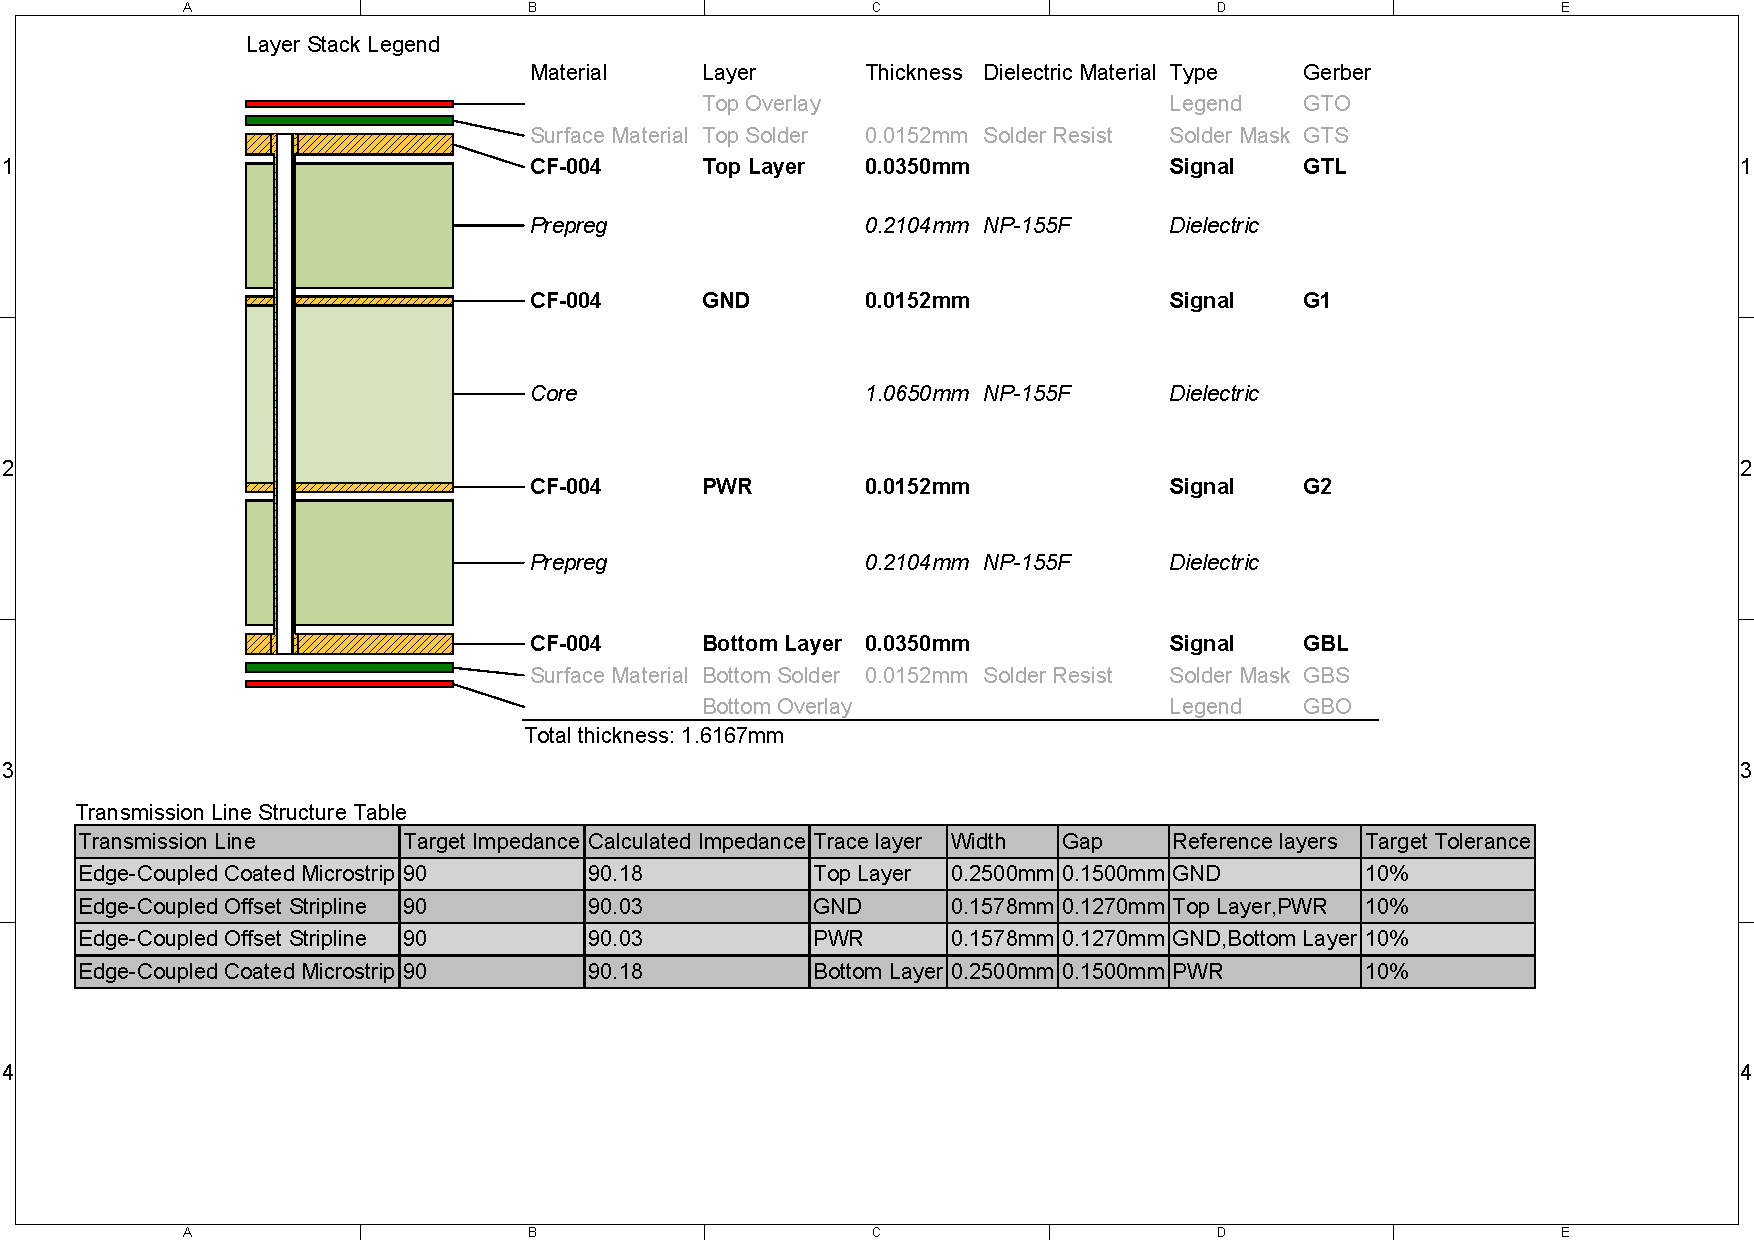
\includegraphics[width=0.75\textwidth, trim=28 114 100 12, clip]{BYTE_SPIne_Stackup.pdf}
\caption{Layer stack and differential impedance profile (Altium Draftsman). The USB pairs
(\qty{0.25}{mm} width, \qty{0.15}{mm} gap) are routed only on L1 and L4, where they reach \qty{90.18}{\ohm} (target
\qty{90}{\ohm} $\pm\qty{10}{\percent}$). The inner-layer rows belong to the same profile but are not used.}
\label{fig:stackup}
\end{figure}

\subsection{Board Outline and Floorplan}

The board measures about $108 \times \qty{73}{mm}$ with four plated M3 mounting holes (\qty{3.2}{mm} drill, \qty{6}{mm}
pad, eight stitching pads) placed \qty{3.5}{mm} from the edges and connected to GND.

A butterfly arrangement ($2{\times}2$ channels around a central header) was evaluated first and
discarded: the ribbon cable would leave the centre of the board vertically, and the motor wiring
would exit on two opposite sides. The final floorplan is \textbf{linear ($1{\times}4$)}, with a single signal flow
from the Jetson side to the motor side:

\begin{figure}[H]
\centering
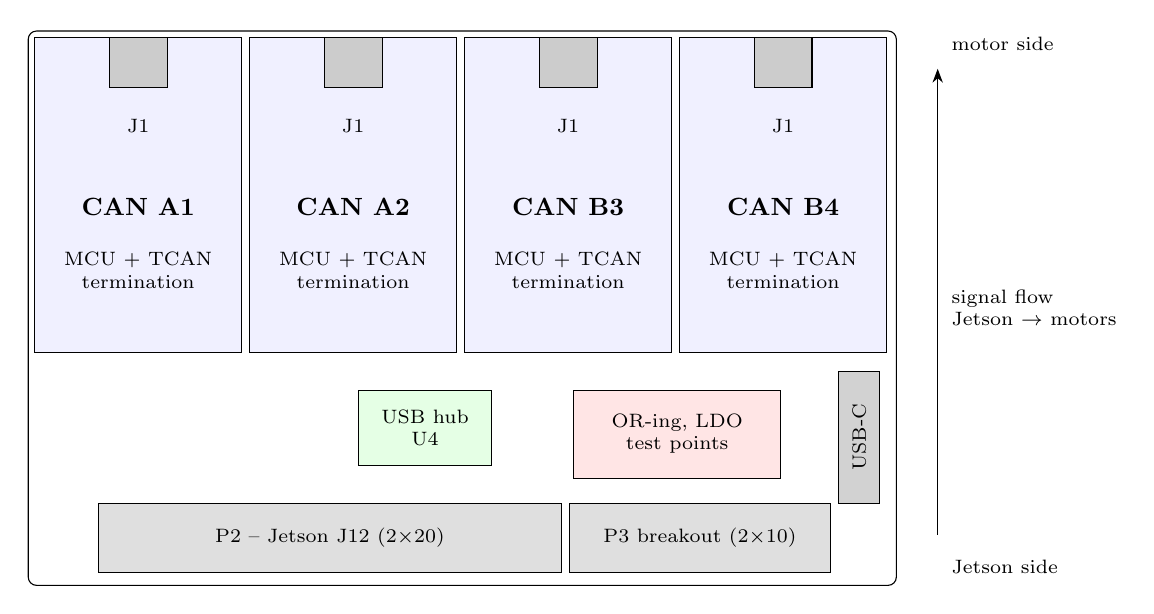
\begin{tikzpicture}[font=\scriptsize, x=1.05cm, y=1.6cm]
    \draw[rounded corners=3pt] (0,0) rectangle (10.5,4.4);
    \foreach \i/\name in {0/A1, 1/A2, 2/B3, 3/B4} {
        \pgfmathsetmacro{\x}{0.08 + \i*2.6}
        \draw[fill=blue!6] (\x,1.85) rectangle ++(2.5,2.5);
        \draw[fill=gray!40] (\x+0.9,3.95) rectangle ++(0.7,0.4);
        \node at (\x+1.25,3.65) {J1};
        \node at (\x+1.25,3.0) {\small\textbf{CAN \name}};
        \node[align=center] at (\x+1.25,2.5) {MCU + TCAN\\termination};
    }
    \draw[fill=green!10] (4.0,0.95) rectangle ++(1.6,0.6) node[midway, align=center] {USB hub\\U4};
    \draw[fill=red!10] (6.6,0.85) rectangle ++(2.5,0.7) node[midway, align=center] {OR-ing, LDO\\test points};
    \draw[fill=gray!35] (9.8,0.65) rectangle ++(0.5,1.05) node[midway, rotate=90] {USB-C};
    \draw[fill=gray!25] (0.85,0.1) rectangle ++(5.6,0.55) node[midway] {P2 -- Jetson J12 ($2{\times}20$)};
    \draw[fill=gray!25] (6.55,0.1) rectangle ++(3.15,0.55) node[midway] {P3 breakout ($2{\times}10$)};

    \draw[-{Stealth[length=5pt]}] (11.0,0.4) -- (11.0,4.1);
    \node[anchor=west] at (11.05,4.3) {motor side};
    \node[anchor=west] at (11.05,0.15) {Jetson side};
    \node[anchor=west, align=left] at (11.05,2.2) {signal flow\\Jetson $\to$ motors};
\end{tikzpicture}
\caption{Floorplan (schematic, not to scale in detail). The four identical channels are placed in
a row; the Jetson header, the breakout, the hub and the power stage share the bottom strip; the
CAN connectors are on the top edge.}
\label{fig:floorplan}
\end{figure}

This arrangement keeps the clean Jetson/USB side and the noisy motor-cable side on opposite
edges, lets all four channels have the same orientation, and allows the routing of one channel to
be replicated on the others with \textit{Copy Room Formats} without rotation.

\subsection{Channel Placement}

In every channel the MCU is oriented so that its pins face the parts they connect to: the SPI
and USB pins face the bottom strip (P2 and the hub), and the CAN pins face the transceiver
and the J1 connector. This keeps the tracks short and avoids crossings around the MCU:

\begin{table}[H]
\centering
\begin{tabular}{ll>{\raggedright\arraybackslash}p{0.66\textwidth}}
\toprule
MCU side & Pins & Signals \\
\midrule
Bottom & 25--36 & SPI2 (25--28), USB PA11/PA12 (32, 33), SWDIO (34), VDDIO2 (36) -- towards P2 and the hub \\
Right  & 37--48 & SWCLK (37), BOOT0 (44), CAN PB8/PB9 (45, 46), VDD (48) -- towards the transceiver \\
Top    & 1--12  & VBAT (1), crystal PF0/PF1 (5, 6), NRST (7), VDDA (9), LEDs PA0/PA1 (10, 11) \\
Left   & 13--24 & SPI\_INT PB11 (22), VDD (24) \\
\bottomrule
\end{tabular}
\caption{Sides of the MCU in the chosen orientation.}
\label{tab:mcusides}
\end{table}

Placement priorities around the MCU:
\begin{enumerate}
    \item \qty{100}{nF} decoupling capacitors at their VDD pins, with the via placed \textit{after} the capacitor
    pad (pin $\to$ capacitor $\to$ via);
    \item crystal Y1 directly in front of PF0/PF1 with C7/C8 beside it; no other track under or next
    to the oscillator. The two crystal tracks do not need to be equal in length: they are two
    different nodes of a Pierce oscillator, and a difference of a few millimetres adds only tenths
    of a picofarad;
    \item C11/C12 on VDDA, then C4 on NRST (second row, NRST track leaving away from the
    crystal);
    \item R10 next to BOOT0; R5 (STB pull-down) near the transceiver, its track kept away from
    CANH/CANL.
\end{enumerate}

The TCAN1042 is placed to the right of the MCU, with pins 1--4 (TXD, GND, VCC, RXD)
facing the MCU and pins 5--8 facing the bus side. The bus path is J1 $\to$ PESD1CAN $\to$ split
termination $\to$ transceiver; the termination resistors are shunt elements and do not lengthen
the signal path. CANH and CANL are routed around the $2{\times}2$ termination block and differ by
\qty{5.1}{mm} (24.1 vs \qty{29.2}{mm}), i.e.\ about \qty{19}{ps}, which is negligible against the \qty{1}{\micro s} bit time.

\subsection{Design Rules}

\begin{table}[H]
\centering
\begin{tabular}{l>{\raggedright\arraybackslash}p{0.6\textwidth}}
\toprule
Rule & Value \\
\midrule
Clearance & \qty{0.15}{mm} (the \qty{0.5}{mm} pitch of the LQFP48 and USB-C leaves \qty{0.2}{mm} between pads) \\
Track width (default) & min 0.15, preferred 0.254, max \qty{1}{mm} \\
Track width \net{3V3}, \net{GND} & min 0.2, preferred \qty{0.3}{mm} \\
Track width \net{5V}, \net{5VUSB}, \net{5V\_SPI} & min 0.3, preferred \qty{0.6}{mm} \\
Vias & \qty{0.3}{mm} drill, \qty{0.6}{mm} diameter, tented on both sides in the design and manufactured
as plugged vias (JLCPCB no longer offers tented vias); minimum annular ring \qty{0.1}{mm} \\
Differential pairs (USB) & width \qty{0.25}{mm}, gap \qty{0.15}{mm} (\qty{90.2}{\ohm} differential, Figure~\ref{fig:stackup}),
max uncoupled length \qty{5}{mm} \\
Polygon connection & THT pads: relief (hand soldering); SMD pads and vias: direct \\
Solder mask sliver & \qty{0.1}{mm}; maximum hole size \qty{3.5}{mm} (M3 holes) \\
Copper to board edge & \qty{0.3}{mm} (JLCPCB minimum \qty{0.2}{mm}, \qtyrange{0.3}{0.5}{mm} recommended for reliability) \\
Bottom GND pour clearance & \qty{0.3}{mm} (\texttt{InPolygon and OnLayer('Bottom Layer')}); the inner planes keep
\qty{0.15}{mm} so that via antipads do not merge into slots \\
\bottomrule
\end{tabular}
\caption{Main design rules (JLCPCB 4-layer capabilities with margin).}
\label{tab:rules}
\end{table}

\subsection{Signal Integrity Considerations}\label{sec:si}

A track behaves as a transmission line only when it is longer than about one sixth of the distance
travelled by a signal edge (\qty{6.5}{ps/mm} on FR4):
\begin{equation}
l_\text{crit} = \frac{t_r}{6 \cdot \qty{6.5}{ps/mm}}
\end{equation}
What matters is the edge time of the \textit{driver}, not the clock frequency. The SPI lines have two
different drivers: MISO is driven by the STM32, configured at low output speed, while SCK,
MOSI and NSS are driven by the TXB0108 translators of the Jetson carrier board, whose output
edges are much faster:

\begin{table}[H]
\centering
\begin{tabular}{llccc}
\toprule
Signal & Driver & Edge time & Critical length & Longest track \\
\midrule
CAN, \qty{1}{Mbit/s} & TCAN1042 & \qtyrange{20}{50}{ns} & $>\qty{500}{mm}$ & $\approx\qty{30}{mm}$ \\
SPI MISO & STM32, low speed & $\approx\qty{12}{ns}$ & $\approx\qty{300}{mm}$ & $<\qty{112}{mm}$ \\
SPI SCK, MOSI, NSS & TXB0108 (Jetson) & \qtyrange{0.6}{2.5}{ns} & \qtyrange{15}{64}{mm} & \qty{112}{mm} \\
\bottomrule
\end{tabular}
\caption{Critical lengths. CAN and MISO are electrically short; the lines driven by the Jetson
are transmission lines and were checked with a reflection simulation (\sireport).}
\label{tab:lcrit}
\end{table}

An earlier version of this table assumed SPI edges of \qtyrange{5}{10}{ns} for all lines (critical length
above \qty{130}{mm}). That assumption holds for MISO only; the simulation showed that it does not
hold for the lines driven by the TXB0108. Controlled impedance is still not required for the SPI
lines: their reflections are controlled with series terminations at the drivers (see below). Only
the USB pairs are routed as \qty{90}{\ohm} differential pairs, which is good practice rather than a necessity
at Full Speed (\qty{12}{Mbit/s}). The field solver gives \qty{90.18}{\ohm} for the routed geometry on both outer
layers, well within the $\pm\qty{10}{\percent}$ tolerance (Figure~\ref{fig:stackup}).

\paragraph{SPI.} SCK, MOSI and MISO of the two MCUs of a bus join at the pads of P2 (star topology).
On SPI1 the pins are spread over the whole header (MOSI on pin 37, SCK on pin 13), so SPI1
MOSI is the longest line (\qty{112}{mm}). Its capacitive load (Jetson carrier, ribbon, PCB track and
two MCU inputs, about \qty{40}{pF}) is within the range recommended for the TXB0108 translators;
widening the track would only increase it. SPI lines are spaced \qty{1}{mm} centre-to-centre ($\approx 3\times$ the
track width). Where NSS runs next to SCK for a few millimetres (at USB crossings) the coupled
glitch is estimated at \qtyrange{10}{15}{mV}, far below the $\approx\qty{1}{V}$ input threshold. The SPI GPIOs
(and SPI\_INT) must be configured at low output speed in the firmware.

\paragraph{SPI simulation and SCK series resistors.} The reflections of the SPI1 bus were simulated
with the Altium Signal Integrity analyser on the routed board, using the IBIS models of the
STM32F072 and of the TXB0108 (fastest driver model, i.e.\ worst case). The complete procedure,
the models and all waveforms are in the separate \sireport{} (Section 3); the results are
summarised here. Thresholds: STM32 $V_{IL}/V_{IH} = 0.99/\qty{2.31}{V}$, TXB0108 $1.05/\qty{2.34}{V}$.

\begin{table}[H]
\centering
\begin{tabular}{llc>{\raggedright\arraybackslash}p{0.3\textwidth}}
\toprule
Net & Worst receiver & Min.\ after rising edge & Result \\
\midrule
MISO (R4 at the driver) & P2-22 (Jetson) & \qty{2.77}{V} & pass, margin \qty{0.43}{V} \\
MOSI & MCU B4 & \qty{1.60}{V} & re-enters the threshold band for $\approx\qty{20}{ns}$ after the edge; acceptable
for a data line, which is sampled \qtyrange{125}{500}{ns} later \\
SCK, no resistor & MCU B4 & \qty{2.09}{V} & marginal: \qty{0.22}{V} below $V_{IH}$ on the clock line \\
\textbf{SCK, \qty{33}{\ohm}} & MCU B4 & \qty{2.79}{V} & \textbf{pass}, margin \qty{0.48}{V}; peak reduced from 4.9 to \qty{4.1}{V} \\
\bottomrule
\end{tabular}
\caption{SPI1 reflection results (\sireport, Table 14). The SCK result with \qty{33}{\ohm} is the
analysis of the final layout.}
\label{tab:sires}
\end{table}

As a result of the simulation (\sireport, Section 3.8 and Figure 4), a \qty{33}{\ohm} series resistor
was added on each clock line: \textbf{R17 on SPI1\_SCK (P2 pin 13) and R18 on SPI0\_SCK
(P2 pin 23)}. A source termination only works close to the driver, so both are placed on the
top layer within \qtyrange{3}{5}{mm} of the P2 pad and \textit{before} the branch point of the star; the branch
point is a via next to the resistor, from which the bottom-layer branch leaves. The part is the
same as R4 (\texttt{C23140}, Basic), so no BOM line and no setup fee are added. The time constant
$\qty{33}{\ohm} \times \qty{40}{pF} \approx \qty{1.3}{ns}$ is negligible at \qtyrange{1}{4}{MHz}. SPI0 was not simulated: it has the same
star topology at P2 and is treated by similarity. The simulation does not include the track of
the Jetson carrier nor the ribbon cable, so SCK must be checked with an oscilloscope on the
prototype with the final cable (Section~\ref{sec:next}).

\paragraph{USB.} Five pairs are routed: J2 $\to$ U3 $\to$ U4 (upstream) and U4 $\to$ MCU (four downstream
ports). The downstream pins of the SL2.1A (DM4, DP4 \dots\ DM1, DP1 on pins 1--8) face the
MCUs in mirrored order with respect to PA11/PA12, and D+/D$-$ cannot be swapped in USB.
Each pair is therefore swapped with one line passing under the other on the bottom layer (two
vias). For the channels whose pair also has to cross an SPI bundle, the swap is combined with the
crossing: both lines go down, cross under the SPI lines, and come back up at two different points
(four vias in total instead of six). The resulting skew of \qtyrange{1}{2}{mm} ($\approx\qty{13}{ps}$) is negligible
against the \qty{83}{ns} bit time. The bottom-layer sections are kept over the continuous \qty{3.3}{V} area of
L3.

\subsection{Power Distribution}

\begin{itemize}
    \item \textbf{L2} is a solid GND pour over the whole board, never split.
    \item \textbf{L3} is a \qty{3.3}{V} pour. The \qty{5}{V} supply of the four transceivers is routed inside it as a \textbf{tree} of
    \qty{1}{mm} tracks starting at the OR-ing output, with one branch per transceiver. The branches
    are not joined at the top: a closed ring would isolate islands of the \qty{3.3}{V} plane. Bottom-layer
    signals do not cross the \qty{5}{V} tracks.
    \item Voltage drop on the longest branch (\qty{67}{mm}, \qty{1}{mm} wide, \qty{15.2}{\micro m} copper): $R = \rho L/(w\,t) \approx
    \qty{76}{m\ohm}$, i.e.\ \qtyrange{5}{11}{mV} at \qtyrange{70}{140}{mA}. The transceivers therefore receive about
    \qty{4.69}{V} even with a \qty{4.75}{V} source, above the \qty{4.5}{V} minimum.
    \item \net{5V\_SPI} (P2 pins 2 and 4, joined) is routed on L3 with a width of at least \qty{0.8}{mm}: according
    to IPC-2221~\cite{ipc2221} an inner 0.5\,oz track needs about \qty{0.7}{mm} for \qty{0.5}{A} with a \qty{10}{\degreeCelsius}
    temperature rise. Layer transitions use two or three vias (about \qty{1}{A} each).
    \item Small top-layer pours connect the OR-ing (\net{5V\_SPI}, \net{5VUSB}, \net{5V} kept as separate nets) and
    the AMS1117 output (tab, pin 2, C21, TP1), with thermal vias to the \qty{3.3}{V} plane. Small
    pours are poured before the large planes (pour order), so that the planes flow around them.
    \item \net{3V3\_Jetson} is a separate net routed only as a track to P3; it never touches the \qty{3.3}{V} plane.
    \item \textbf{L4} carries a GND pour over the whole board, stitched to L2 with GND vias (about every
    \qtyrange{5}{10}{mm}, along the edges, at the end of narrow copper fingers and next to the signal
    vias of the bottom-layer crossings). It gives the bottom-layer tracks a nearby GND return
    and improves the copper balance. No pour was added on the top layer: there the free
    copper is fragmented between components and would create many small, poorly stitched
    areas, with little benefit over the solid GND plane on L2.
\end{itemize}

The \qty{3.3}{V} pour on L3 was checked after all pours and stitching vias: it remains a single connected
area (no island is isolated by the \qty{5}{V} tree or by via antipads). Since L3 is a signal-type layer
with a polygon, Altium's automatic via stitching is blocked by the \qty{3.3}{V} polygon; the stitching
vias were therefore placed manually.

% ---------------------------------------------------------------------------
\section{Conclusion and Recommendations}

The BYTE SPIne provides four independent CAN buses for the twelve actuators of the BARK
quadruped, with one MCU and one transceiver per leg. The same hardware supports a ready-to-use
USB/candleLight mode and the final SPI mode, so development can start immediately
without a second board revision.

The key sizing choices are:
\begin{itemize}
    \item an external \qty{8}{MHz} crystal per MCU, required for CAN timing without USB;
    \item a split termination built from $2\times\qty{120}{\ohm}$ 1206 per half, sized for the \qty{100}{mA} fault current
    of the transceiver;
    \item an ideal-diode OR-ing (LM66100, figure 17 configuration) that keeps the \qty{5}{V} rail above the
    \qty{4.5}{V} minimum of the TCAN1042;
    \item a \qty{100}{k\ohm} NSS pull-up, compatible with the TXB0108 translators of the Jetson;
    \item \qty{33}{\ohm} source terminations on MISO (R4) and, as a result of the signal integrity simulation,
    on both SCK lines (R17, R18).
\end{itemize}
The USB mode has been tested and validated on the prototype and works without errors
(status of 26 November 2026). The SPI mode has not been tested yet; its reliability depends
mainly on the firmware.

\required{implement the MCU-side CAN loop, the \textbf{CRC and sequence counter} on SPI
packets and the \textbf{communication watchdog} before the robot is operated in SPI mode.}

\section{Next Steps for future iterations}\label{sec:next}

\begin{itemize}
    \item Bench validation of the prototype (version 1.0):
    \begin{itemize}[label=--]
        \item \textbf{done (26 November 2026):} USB mode with candleLight, tested and validated: the board
        works without errors;
        \item \textbf{SPI mode, not yet tested:} MISO release with two MCUs on the same SPI bus;
        \item \textbf{SPI mode, not yet tested:} SCK at both MCUs of a bus with an oscilloscope (short ground
        spring), with the final ribbon cable, to confirm the simulation;
        \item \textbf{SPI mode, not yet tested:} SPI link at \qty{1}{kHz} for 10 minutes with zero lost packets
        (sequence counter and CRC);
        \item to be measured and documented: stability of the \qty{3.3}{V} rail with the ceramic output capacitor;
        \qty{5}{V} rail voltage under full CAN load, from both sources;
        \item pinout of the CAN cables (\texttt{H L G}) against the SteadyWin connector.
    \end{itemize}
    \item Remaining simulations (\sireport, Section 5): SCK with the realistic TXB0108 model,
    NSS falling edge, crosstalk SCK $\to$ NSS, SPI0 on the layout.
    \item Version 1.1: fixes resulting from the bench tests; schematic clean-up (electrical type of the
    supply pins of the TCAN1042 and SL2.1A symbols, one single name for the \net{5VUSB} net).
    \item Optional improvement: a right-angle version of P2 would let the ribbon cable leave parallel
    to the board.
    \item Firmware: candleLight build for the BYTE SPIne pinout (done, patch in
    \texttt{BYTE\_SPIne/Firmware/BYTE\_SPIne\_candleLight.patch}); SPI slave firmware with watchdog
    (not yet tested).
    \item Verify the termination of the actuators (only the last motor of each leg terminated).
\end{itemize}

\section{Annexes}

Complete schematic of the BYTE SPIne (\href{run:BYTE_SPIne_Schematic.pdf}{\texttt{BYTE\_SPIne\_Schematic.pdf}}, generated by the Output
Job of the project): top sheet, one CAN channel (instantiated four times) and USB hub.

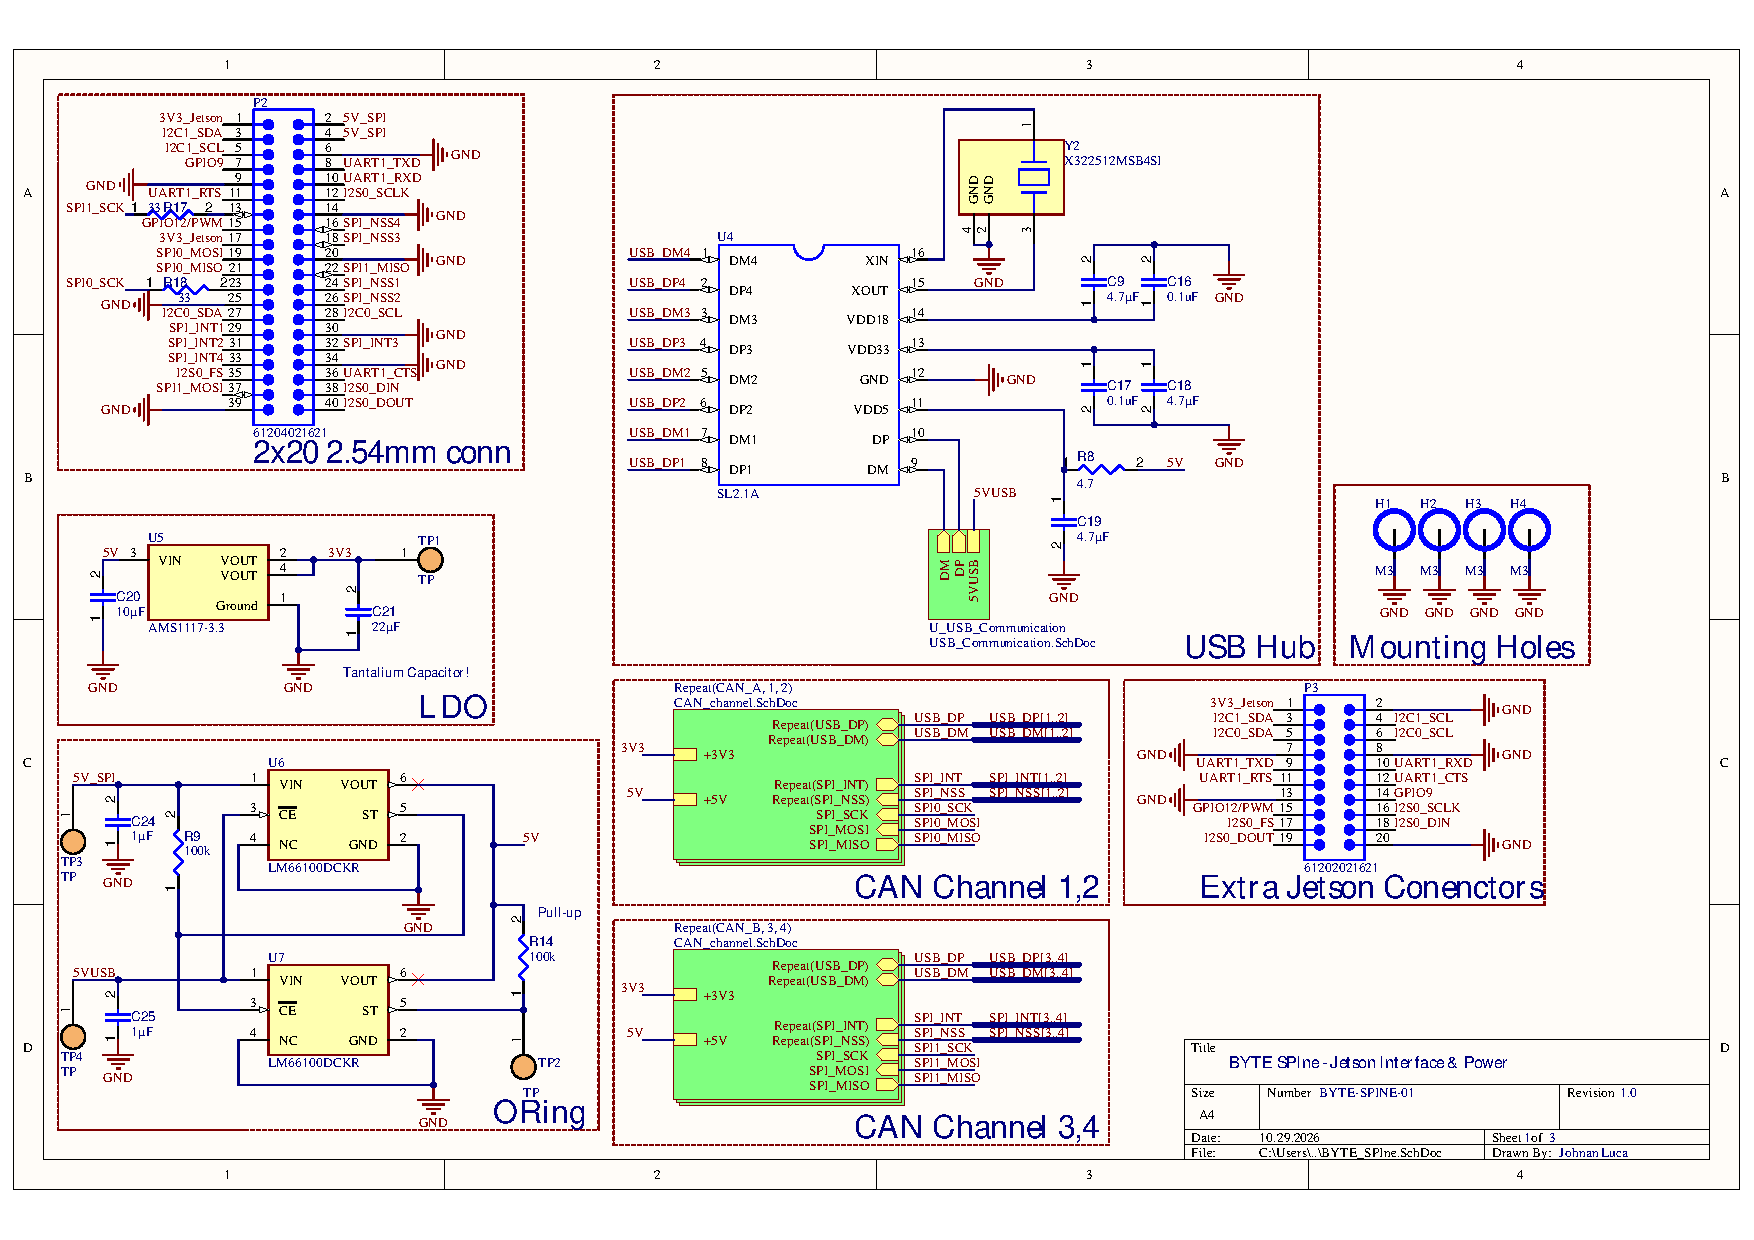
\includepdf[pages=-, fitpaper=true]{BYTE_SPIne_Schematic.pdf}

\section{References}

{\renewcommand{\section}[2]{}%
\begin{thebibliography}{99}
\bibitem{stm32} STMicroelectronics, \textit{STM32F072x8/xB datasheet}, DocID025004. Product page with
datasheet, reference manual and application notes: \url{https://www.st.com/en/microcontrollers-microprocessors/stm32f072c8.html}.
\bibitem{tcan} Texas Instruments, \textit{TCAN1042H, TCAN1042HG, TCAN1042HGV, TCAN1042HV
datasheet}, SLLSES7D, October 2021, \url{https://www.ti.com/document-viewer/TCAN1042H/datasheet}.
\bibitem{sl21a} Shenzhen CoreChips Microelectronics, \textit{SL2.1A USB 2.0 high-speed 4-port hub controller
datasheet}, V4.0, \url{https://wmsc.lcsc.com/wmsc/upload/file/pdf/v2/lcsc/CoreChips-SL2-1A_C192893.pdf}; part used on the board:
\url{https://jlcpcb.com/partdetail/CoreChips-SL21A/C6798314}.
\bibitem{ams1117} Advanced Monolithic Systems, \textit{AMS1117 1A low dropout voltage regulator datasheet},
\url{http://www.advanced-monolithic.com/pdf/ds1117.pdf}.
\bibitem{lm66100} Texas Instruments, \textit{LM66100 5.5-V, 1.5-A ideal diode datasheet},
\url{https://www.ti.com/lit/ds/symlink/lm66100.pdf}.
\bibitem{pesd} Nexperia, \textit{PESD1CAN CAN bus ESD protection diode datasheet},
\url{https://assets.nexperia.com/documents/data-sheet/PESD1CAN.pdf}.
\bibitem{jetson} NVIDIA, \textit{Jetson Orin Nano Developer Kit Carrier Board Specification}, SP-11324-001, v1.3,
Jetson Download Center (NVIDIA account required): \url{https://developer.nvidia.com/embedded/downloads}; developer kit user guide:
\url{https://developer.nvidia.com/embedded/learn/jetson-orin-nano-devkit-user-guide/index.html}.
\bibitem{txb} Texas Instruments, \textit{TXB0108 8-bit bidirectional voltage-level translator datasheet},
\url{https://www.ti.com/product/TXB0108}.
\bibitem{steadywin} SteadyWin, \textit{SteadyWin Motor Driver Protocol Specification (GIM series actuators)}, provided
by the manufacturer with the actuators; no public link available.
\bibitem{candlelight} candle-usb, \textit{candleLight\_fw}, \url{https://github.com/candle-usb/candleLight_fw}.
\bibitem{jetsonhacks} JetsonHacks, \textit{NVIDIA Jetson Orin Nano GPIO header pinout},
\url{https://jetsonhacks.com/nvidia-jetson-orin-nano-gpio-header-pinout/}.
\bibitem{jlcparts} JLCPCB, \textit{Parts library (Basic and Extended parts)}, \url{https://jlcpcb.com/parts}.
\bibitem{an2867} STMicroelectronics, \textit{AN2867 -- Oscillator design guide for STM32 microcontrollers},
\url{https://www.st.com/resource/en/application_note/an2867-oscillator-design-guide-for-stm32-microcontrollers-stmicroelectronics.pdf}.
\bibitem{an4080} STMicroelectronics, \textit{AN4080 -- Getting started with STM32F0x1/x2/x8 hardware development},
listed in the documentation of the product page: \url{https://www.st.com/en/microcontrollers-microprocessors/stm32f072c8.html}.
\bibitem{ipc2221} IPC, \textit{IPC-2221 Generic Standard on Printed Board Design} (conductor sizing); paid standard,
\url{https://www.ipc.org}.
\bibitem{jlcstack} JLCPCB, \textit{JLC04161H-7628 4-layer impedance stack-up and PCB manufacturing capabilities},
\url{https://jlcpcb.com/capabilities/pcb-capabilities}.
\bibitem{si} J. Luca, \textit{Impedance and Signal Integrity Simulation of the BYTE SPIne SPI-to-CAN Bridge},
companion report, \texttt{Documentation/BYTE\_SPIne\_SI\_Simulation.pdf}, October 2026.
\end{thebibliography}}

\end{document}
